% =============================================================================
%  supp_acmmm.tex  --  Supplementary Material for "Rank Before You Merge"
%  Converted from drafts/supp_acmmm.md (S1--S9). Double-blind.
%
%  S1/S2 TODO COMPLETION (this build):
%   - S1 Kendall-tau column filled from drafts/paper_v4.md Sec. 4.1 (M1 table):
%       DocVQA 0.094, TextVQA 0.227, GQA 0.249.
%   - S2 per-benchmark Sobel cells filled from drafts/paper_v4.md Sec. 4.2 (M2
%       table): TextVQA 0.281/0.186, 72% vs 53%; GQA 0.304/0.271, 58% vs 53%.
%     All values exist in paper_v4 -> NO "[TODO source missing]" remains.
%   Source of the filled cells = the same M1/M2 mechanism campaign
%   (mechanism_verification_report Sec. 1--2; released with code).
%
%  Numbers are copied verbatim. Run/digest paths are reproducibility metadata
%  (generic internal filenames; they identify no author / repo / institution).
% =============================================================================

\documentclass[sigconf,review,anonymous]{acmart}

\usepackage{booktabs}
\usepackage{multirow}
\usepackage{pifont}     % \ding{51}=check
\usepackage{graphicx}
\usepackage{url}        % \path{} for run/digest paths

\setcopyright{none}
\settopmatter{printacmref=false, printccs=false, printfolios=true}

\begin{document}

\title[Rank Before You Merge: Supplementary Material]{Supplementary Material --- Rank Before You Merge: A Stage Law for
  Training-Free Visual Token Compression in Merger-Equipped Vision-Language
  Models}

\author{Anonymous Author(s)}
\affiliation{\institution{Anonymous Affiliation}\country{}}

\maketitle

\noindent\footnotesize Every number is labeled with its source digest
(\path{experiments/*.md}) or run-JSON path. Tables S1--S3/S7 support
\S\,5 of the body; S4--S6 support \S\,4 (S4b cascade counts support \S\,6); S8
supports \S\,3; S9 is the per-cell reproducibility index, with the full
per-cell listing (cell / $n$ / official / ptid / skip / JSON path) in
S9.1--S9.4; S10 is a qualitative same-image pre/post selection comparison
rendered from measured Qwen3-VL-8B merger L2 (four panels each, no paired
question); S11 reports the fourth-family GLM-4.1V gate and decoding diagnostic.

% =============================================================================
\section*{S1. M1 --- merger ranking reshuffle, full table (Qwen3-VL-8B, seed-0, $n = 64$/benchmark)}
% =============================================================================

Per image, Spearman correlation of the pre ranking (merger-input unit L2) with
the post ranking (merged-token L2) over all units, plus top-25\% kept-set
overlap. Source: mechanism\_verification\_report \S\,1 (M1 campaign; released
with code) via \path{drafts/paper_v4.md} \S\,4 (measured under the
\path{experiments/j3_mechanism_crossarch.md} campaign). The Kendall-$\tau$
column is taken from the same M1 table in \path{drafts/paper_v4.md} \S\,4.1.

\begin{table}[h]
  \centering
  \small
  \begin{tabular}{@{}l r r r@{}}
    \toprule
    Benchmark (type) & Spearman $\rho$ & Jaccard@25\% & Kendall $\tau$ \\
    \midrule
    DocVQA (text-dense document) & \textbf{0.137} & \textbf{0.180} & 0.094 \\
    TextVQA (text-dense scene)   & 0.332          & 0.243          & 0.227 \\
    GQA (object-centric)         & \textbf{0.360} & \textbf{0.278} & 0.249 \\
    \bottomrule
  \end{tabular}
\end{table}

\noindent\textbf{Reading:} the reshuffle is largest on the most text-dense
benchmark and smallest (but still substantial) on object-centric GQA ---
$\rho = 0.137 < 0.332 < 0.360$; Jaccard $= 0.180 < 0.243 < 0.278$. Chance-level
Jaccard at $\kappa = 25\%$ is 0.25 (overlap is below random for DocVQA, i.e.\
actively anti-correlated in the decision band).

% =============================================================================
\section*{S2. M2 --- demotion directionality vs text-stroke energy, full table (same sample as S1)}
% =============================================================================

rank\_shift $=$ post\_rank $-$ pre\_rank ($+$ $\Rightarrow$ demoted); per-unit
Sobel edge energy as the text-stroke proxy. Source: mechanism\_verification\_report
\S\,2 (M2 campaign; released with code) via \path{drafts/paper_v4.md} \S\,4.
The per-benchmark Sobel means and median fractions (TextVQA, GQA) are taken
from the same M2 table in \path{drafts/paper_v4.md} \S\,4.2.

\begin{table}[h]
  \centering
  \small
  \begin{tabular}{@{}l r r r l@{}}
    \toprule
    Benchmark & $\rho$(rank\_shift, Sobel edge) & mean Sobel, post-drops-pre-keeps & mean Sobel, reverse group & \% demoted above per-image median \\
    \midrule
    DocVQA  & \textbf{+0.439} & \textbf{0.641} & 0.124 & \textbf{92\% (vs 35\%)} \\
    TextVQA & +0.155          & 0.281          & 0.186 & 72\% (vs 53\%) \\
    GQA     & +0.036          & 0.304          & 0.271 & 58\% (vs 53\%) \\
    \bottomrule
  \end{tabular}
\end{table}

\noindent\textbf{Reading:} the merger preferentially demotes high-edge
(text-stroke) units ${\sim}12\times$ more strongly on documents than on object
scenes; on DocVQA the units post drops that pre keeps are the highest-edge of
all (92\% above the per-image median vs 35\% for the reverse group) ---
post-merger selection is systematically anti-text on documents. Directionality
hypothesis (merger trained on natural content attenuates high-frequency stroke
energy): testable hypothesis, not a measured result. Second text-stroke proxy
(Laplacian variance): future work (single-proxy disclosure).

% =============================================================================
\section*{S3. Retention curve --- full number strings ($n = 200$, both Qwen models)}
% =============================================================================

pre$-$post $\Delta$ at 75\% / 50\% / 25\% retention (the body \S\,5.4 prints
endpoints only). Source: \path{experiments/j8_ablations.md} via
\path{drafts/paper_v4.md} \S\,5.6.

\begin{table}[h]
  \centering
  \small
  \begin{tabular}{@{}l l r r r@{}}
    \toprule
    Model & Benchmark & $\Delta$ @75\% & $\Delta$ @50\% & $\Delta$ @25\% \\
    \midrule
    Qwen3-VL-8B   & TextVQA & $+8.7$ pp  & $+29.0$ pp & \textbf{+38.4 pp} \\
    Qwen3-VL-8B   & DocVQA  & $-1.3$ pp  & $+5.9$ pp  & \textbf{+24.3 pp} \\
    Qwen2.5-VL-7B & TextVQA & $+7.0$ pp  & $+15.3$ pp & \textbf{+26.1 pp} \\
    Qwen2.5-VL-7B & DocVQA  & $-2.1$ pp  & $-1.4$ pp  & \textbf{+11.0 pp} \\
    \bottomrule
  \end{tabular}
\end{table}

\noindent\textbf{Reading:} the two stages are indistinguishable under shallow
compression (DocVQA post even leads 1--2~pp within noise at 75\%); the
pre-merger lead emerges and widens monotonically with depth. Same shallow
regime as the GQA sign and the Qwen2.5-VL 600k-cap reversal (body \S\,5.4
boundary; \S\,8 item~3). Data source for Fig.~3.

% =============================================================================
\section*{S4. Primary paired McNemar statistics --- per cell (full splits, both Qwen models)}
% =============================================================================

Primary test $=$ paired McNemar $z$ on per-sample correctness,
$z = (b - c)/\sqrt{b + c}$, with $b/c$ the pre-only / post-only correct counts;
positive $z =$ pre-merger lead, negative $=$ post-merger lead (GQA only).
Cross-check $=$ independent-binomial $z$ (SE $\sqrt{\mathrm{se}^2_{\mathrm{pre}}
+ \mathrm{se}^2_{\mathrm{post}}}$); ``agree \%'' $=$ per-question agreement of
the recorded correctness indicators. Source: \path{drafts/paper_v4.md} \S\,5.2
paired-test table (per-sample rescore of \path{runs/full_matrix/j7_*_full.json},
paired by question id, restricted to ids answered in both arms; 200/200
ground-truth self-test) + \path{experiments/j7_main_table.md}.

\begin{table*}[h]
  \centering
  \small
  \begin{tabular}{@{}l l c l r r r r r@{}}
    \toprule
    Model & Benchmark & $\kappa$ & $\Delta$ (official) & McNemar $z$ (primary) & $b$ (pre-only) & $c$ (post-only) & agree \% & indep-binom $z$ \\
    \midrule
    Qwen3-VL-8B   & TextVQA   & .25  & $+38.4$ pp   & \textbf{+43.0} & 2349 & 183  & 49.4 & 42.3 \\
    Qwen3-VL-8B   & DocVQA    & .25  & $+24.3$ pp   & \textbf{+34.7} & 1601 & 150  & 67.3 & 27.1 \\
    Qwen3-VL-8B   & OCR-Bench & .25  & $+363$ pts   & \textbf{+16.7} & 422  & 56   & 52.2 & 18.2 \\
    Qwen3-VL-8B   & GQA       & .25  & $-2.8$ pp \dag & \textbf{$-$8.0} & 834 & 1196 & 83.9 & 4.5 \\
    Qwen3-VL-8B   & TextVQA   & .125 & $+34.0$ pp   & \textbf{+40.8} & 2101 & 161  & 54.8 & 39.9 \\
    Qwen3-VL-8B   & DocVQA    & .125 & $+24.9$ pp   & \textbf{+33.1} & 1437 & 127  & 70.8 & 32.1 \\
    Qwen3-VL-8B   & OCR-Bench & .125 & $+297$ pts   & \textbf{+16.0} & 323  & 25   & 65.2 & 17.8 \\
    \midrule
    Qwen2.5-VL-7B & TextVQA   & .25  & $+26.1$ pp   & \textbf{+30.8} & 1682 & 309  & 60.2 & 27.3 \\
    Qwen2.5-VL-7B & DocVQA    & .25  & $+11.0$ pp   & \textbf{+15.6} & 1406 & 693  & 60.8 & 11.6 \\
    Qwen2.5-VL-7B & OCR-Bench & .25  & $+293$ pts   & \textbf{+14.6} & 347  & 54   & 59.9 & 14.7 \\
    Qwen2.5-VL-7B & GQA       & .25  & $-2.6$ pp \dag & \textbf{$-$5.7} & 892 & 1150 & 83.8 & 4.1 \\
    Qwen2.5-VL-7B & TextVQA   & .125 & $+27.8$ pp   & \textbf{+33.1} & 1836 & 305  & 57.2 & 29.1 \\
    Qwen2.5-VL-7B & DocVQA    & .125 & $+21.0$ pp   & \textbf{+25.6} & 1325 & 294  & 69.7 & 23.3 \\
    Qwen2.5-VL-7B & OCR-Bench & .125 & $+268$ pts   & \textbf{+15.0} & 294  & 26   & 68.0 & 15.9 \\
    \bottomrule
  \end{tabular}
\end{table*}

\noindent\dag\ the only significant post-stage lead. GQA official
word-normalized exact-match rescore gives a concordant McNemar $z = 8.1 / 7.1$
(Qwen3-VL / Qwen2.5-VL). Smallest text-dense $\Delta_{25}$ $|z| = 14.6$
(Qwen2.5-VL OCR-Bench); smallest text-dense $\Delta_{12.5}$ $|z| = 15.0$
(Qwen2.5-VL OCR-Bench); smallest $|z|$ anywhere $= 5.7$ (Qwen2.5-VL GQA). On
OCR-Bench @25\% the independent-binomial cross-check (18.2 / 14.7) marginally
exceeds McNemar (16.7 / 14.6) because the binary correctness indicator coarsens
the /1000 item score (body footnote~e); McNemar remains the primary test and is
$\geq$-consistent on every other cell.

\subsection*{S4b. Cascade two-stage gate --- paired McNemar counts (Qwen3-VL-8B, $n = 200$, official rescore)}

Cascade gate (body Table~5 / \S\,6): single budget, Stage~1 $=$ pre-merger RBM
keeping fraction $X$ of merger-input units, Stage~2 $=$ FastV at LLM layer~2
dropping fraction $Y$ of the survivors; total keep $= X\cdot(1 - Y)$. Three arms
(pre-alone / fastv-alone / cascade) are compared pairwise on identical images
($n_{\mathrm{common}}$ matched; mean post-merger token count identical across
all three arms in every cell, so the comparison is iso-budget). cas\_only /
pre\_only / fst\_only $=$ per-sample counts correct in only the named arm of the
pair. Verdict $=$ NO-GO (cascade fails the Pareto rule on all 8
budget$\times$benchmark cells). Source: \path{runs/cascade/gate_result.json}
(\path{mcnemar_cas_vs_pre} / \path{mcnemar_cas_vs_fst});
\path{experiments/cascade_gate.md}.

\begin{table*}[h]
  \centering
  \footnotesize
  \begin{tabular}{@{}c l r r r r r r r r r r@{}}
    \toprule
    total keep $\kappa$ & bench & $n$ & pre & fst & cas & $z$ (cas vs pre) & cas\_only & pre\_only & $z$ (cas vs fst) & cas\_only & fst\_only \\
    \midrule
    25\%   & TextVQA   & 200 & 0.5967 & 0.6800 & 0.5950 & $-0.152$ & 21 & 22 & $-2.335$ & 18 & 35 \\
    25\%   & DocVQA    & 200 & 0.4239 & 0.5183 & 0.4779 & $+2.066$ & 38 & 22 & $-1.500$ & 26 & 38 \\
    25\%   & OCR-Bench & 181 & 0.5801 & 0.1713 & 0.3978 & $-5.154$ & 4  & 37 & $+6.112$ & 43 & 2 \\
    25\%   & GQA       & 200 & 0.4150 & 0.4900 & 0.4050 & $-0.333$ & 17 & 19 & $-2.429$ & 16 & 33 \\
    \midrule
    12.5\% & TextVQA   & 200 & 0.5000 & 0.4450 & 0.4050 & $-2.540$ & 21 & 41 & $-0.896$ & 27 & 34 \\
    12.5\% & DocVQA    & 200 & 0.2980 & 0.2779 & 0.2070 & $-2.012$ & 31 & 49 & $-2.064$ & 16 & 30 \\
    12.5\% & OCR-Bench & 181 & 0.3591 & 0.0884 & 0.1713 & $-5.013$ & 6  & 40 & $+3.441$ & 17 & 2 \\
    12.5\% & GQA       & 200 & 0.3950 & 0.4550 & 0.3500 & $-1.286$ & 20 & 29 & $-3.130$ & 12 & 33 \\
    \bottomrule
  \end{tabular}
\end{table*}

\noindent\textbf{Reading:} cascade sits strictly between the two single methods
and is dominated by the better arm on every cell --- pre-alone on OCR-Bench
($z = -5.15 / -5.01$ vs pre at 25\% / 12.5\%; the FastV stage destroys exactly
the raw-patch information Stage~1 was built to protect) and FastV-alone on
TextVQA / GQA ($z = -2.34 / -2.43$ vs fst at 25\%). The single positive
cas-vs-pre $z$ (DocVQA 25\%, $+2.07$) is paired with a loss to FastV
($-1.50$), so the ``strictly beats both arms'' condition holds nowhere. Two
training-free selectors composed in series do not complement (body \S\,6).

% =============================================================================
\section*{S5. Binomial stderrs + skip accounting (Table 1 Qwen blocks)}
% =============================================================================

$\sigma = \sqrt{p(1 - p)/n}$, greedy decoding (no temperature variance; error
bars are binomial only). Source: \path{experiments/j7_main_table.md} (stderr
column) + the Qwen-block footnotes of Table~1.

\begin{itemize}
  \item Qwen3-VL none DocVQA: re-run at max-model-len 49,152, native
    resolution, \textbf{0/5349 skips} (ANLS 0.956).
  \item OCR-Bench none cells skip \textbf{18/1000 (Qwen3-VL) / 24/1000
    (Qwen2.5-VL)} long-OCR images on context overrun, scored 0 (conservative);
    compressed cells skip $\leq 5$. The uncompressed anchor is therefore
    understated and the relative gaps are conservative.
  \item Qwen2.5-VL OCR-Bench @25\% RBM: 4~M-pixel cap (mean tokens 229.6 vs
    post 282.0) $\to$ its $+293$-pt gap is conservative (the one iso-token
    exception in the Qwen block of Table~1, note~d).
\end{itemize}

\noindent Per-cell $\sigma$ values (full splits, computed from the printed
official metric $p$ and full-split $n$; greedy decoding $\Rightarrow$ binomial
only):

\begin{table*}[h]
  \centering
  \small
  \begin{tabular}{@{}l l r r r r r r@{}}
    \toprule
    Model & Benchmark & $n$ & none & pre@25\% & post@25\% & pre@12.5\% & post@12.5\% \\
    \midrule
    Qwen3-VL-8B   & TextVQA   & 5000  & 0.0051   & 0.0069 & 0.0059 & 0.0071 & 0.0048 \\
    Qwen3-VL-8B   & DocVQA    & 5349  & --- $^{a}$ & 0.0068 & 0.0058 & 0.0065 & 0.0042 \\
    Qwen3-VL-8B   & OCR-Bench & 1000  & 0.0135   & 0.0157 & 0.0123 & 0.0151 & 0.0071 \\
    Qwen3-VL-8B   & GQA       & 12578 & 0.0043   & 0.0044 & 0.0045 & --- $^{c}$ & --- $^{c}$ \\
    \midrule
    Qwen2.5-VL-7B & TextVQA   & 5000  & 0.0049   & 0.0065 & 0.0070 & 0.0069 & 0.0066 \\
    Qwen2.5-VL-7B & DocVQA    & 5349  & 0.0030   & 0.0066 & 0.0068 & 0.0068 & 0.0059 \\
    Qwen2.5-VL-7B & OCR-Bench & 1000  & 0.0122   & 0.0158 & 0.0122 & 0.0149 & 0.0079 \\
    Qwen2.5-VL-7B & GQA       & 12578 & 0.0044   & 0.0044 & 0.0044 & --- $^{c}$ & --- $^{c}$ \\
    \bottomrule
  \end{tabular}
\end{table*}

\noindent $\sigma = \sqrt{p(1-p)/n}$; each cell's every text-dense
$\Delta_{25}$ is $\geq 15\sigma$ of its own cells' pooled stderr, and the
full-split GQA post lead ($+2.8 / +2.6$~pp) is $\approx 5\sigma$ of the pooled
GQA stderr ($\approx 0.0063$) --- significant but an order of magnitude smaller
than any text-dense $\Delta$. $^{a}$~Qwen3-VL none-DocVQA native-resolution
anchor: full-split run partly skipped on context overrun (re-run at
max-model-len 49,152 gives ANLS 0.956, 0/5349 skips); $\sigma$ not printed for
the partial native cell. $^{c}$~GQA evaluated at $\kappa = 0.25$ only on the
full split (no full-split $\kappa = 0.125$ cells; body footnote~c).

\begin{itemize}
  \item Qwen3-VL OCR-Bench none $= 760/1000$ over 982 attempted (18 skips
    scored 0); compressed @25\%: 547 (pre) / 184 (post), skip $\leq 5$ ---
    ratio $3.0\times$, widening to $6.6\times$ at 12.5\% (350 vs 53).
\end{itemize}

% =============================================================================
\section*{S6. $n = 200$ cross-split consistency (dev-subset vs full-split direction)}
% =============================================================================

The $n = 200$ dev scope used by Tables~3--4 and \S\,5.3 is direction-consistent
with the full splits. Source: \path{experiments/j2_crossgen_matrix.md}
($n = 200$ official) + \path{drafts/paper_v4.md} Table~A2 (j0a/j2/j4 campaigns).
$\Delta_{25} =$ pre $-$ post at $\kappa = 0.25$.

\begin{table}[h]
  \centering
  \small
  \begin{tabular}{@{}l l l l c@{}}
    \toprule
    Model & Benchmark & full-split $\Delta_{25}$ (Table 1) & $n = 200$ $\Delta_{25}$ & same sign? \\
    \midrule
    Qwen3-VL-8B   & TextVQA & $+38.4$ pp & $+38.3$ pp & \ding{51} (pre) \\
    Qwen3-VL-8B   & DocVQA  & $+24.3$ pp & $+26.5$ pp & \ding{51} (pre) \\
    Qwen2.5-VL-7B & TextVQA & $+26.1$ pp & $+32.0$ pp & \ding{51} (pre) \\
    Qwen2.5-VL-7B & DocVQA  & $+11.0$ pp & $+18.8$ pp & \ding{51} (pre) \\
    \bottomrule
  \end{tabular}
\end{table}

\noindent\textbf{Reading:} all four text-dense cells agree in sign (pre-merger
lead) across the two scopes; magnitudes are within run noise (the $n = 200$
subset SE is $\approx 8\times$ larger, so the subset is retained only as a
direction check, never as the headline). The full Qwen3-VL $n = 200$
cross-method view (RBM vs FastV vs Pyramid) and the compact Qwen2.5-VL
$n = 200$ cross-generation matrix are printed in \path{paper_v4} Table~A2 and
\S\,5.4 Table~2 respectively.

% =============================================================================
\section*{S7. Selector invariance (second scorer family, Qwen3-VL)}
% =============================================================================

The stage law under a second, non-L2 scorer (global-centroid attention).
Source: method\_gate\_report via \path{drafts/paper_v4.md} \S\,5 (j3/j5
campaigns).

\begin{table}[h]
  \centering
  \small
  \begin{tabular}{@{}l l r r l@{}}
    \toprule
    Selector & Benchmark & pre & post & $\Delta$ \\
    \midrule
    L2 (paper selector)         & TextVQA                       & 0.598--0.605 & 0.215--0.222 & $\approx +38$ pp \\
    Global-centroid attention   & TextVQA                       & \textbf{0.553} & 0.200 & \textbf{+35.3 pp} \\
    Global-centroid attention   & TextVQA/DocVQA (doubled $n$)  & --- & --- & \textbf{+35.5 / +24.4 pp} \\
    \bottomrule
  \end{tabular}
\end{table}

\noindent\textbf{Reading:} invariant in sign and magnitude on Qwen3-VL --- the
effect is not an L2 artifact. On Qwen2.5-VL the L2 sign is invariant but the
attention proxy degrades (proxy-family specificity, not a counter-example); L2
remains the paper's selector, frozen as plain RBM (\S\,3.2).

% =============================================================================
\section*{S8. Merger tap points and M-RoPE configuration details (supports \S\,3)}
% =============================================================================

\begin{itemize}
  \item \textbf{Qwen3-VL-8B}: first-invoked merger $=$
    \path{deepstack_merger_list[0]} (\path{deepstack_visual_indexes = [8, 16,
    24]}), so unit scores are computed on \textbf{ViT block-8 outputs}
    (intermediate depth); the single resulting mask is shared by all mergers,
    including the main merger that consumes the final-block output. Runner
    diagnostic \path{mask_computed_at = 'deepstack_0'} on every run. Source:
    \path{experiments/r1_1_swap_jaccard.md} Part~B (three-evidence verification:
    call order in \path{Qwen3VLVisionModel.forward}, model config, run
    diagnostics).
  \item \textbf{Qwen2.5-VL-7B}: no deepstack; scores are computed on the
    \textbf{main merger input (final ViT block output)}.
    \path{mask_computed_at = 'main'}.
  \item \textbf{InternVL3-8B}: the pixel-shuffle downsampling stage is the
    merger; L2 taps its input.
  \item \textbf{M-RoPE fix}: Qwen2.5-VL uses a block M-RoPE layout and Qwen3-VL
    an interleaved one; under pruning the position cursor must advance by the
    actual surviving count. A family-scoped fix (bit-degrading to the original
    at full retention) makes the Qwen2.5-VL compression path well-formed; the
    block-vs-interleaved contrast is itself a diagnostic of why naive pruning
    collapses one generation and is tolerated by the other.
  \item \textbf{Table 3 / r2c harness}: HF transformers eager attention,
    \path{--mrope native} (family-agnostic correct positions) on all same-scope
    cells; the Qwen2.5-VL $\times$ pre vllm-mimic positional degeneration
    (repeated ``addCriterion\ldots'' outputs $\to$ pseudo-zero scores) was
    detected and replaced before any reported number; on Qwen3-VL native vs
    mimic give 0.575 vs 0.525 (same ordering). Source:
    \path{experiments/r2c_rbm_scope.md}.
\end{itemize}

% =============================================================================
\section*{S9. Per-cell reproducibility index (run JSONs; gitignored, released with code)}
% =============================================================================

\begin{table*}[h]
  \centering
  \small
  \begin{tabular}{@{}p{3.0cm} c p{4.6cm} p{4.6cm}@{}}
    \toprule
    Body location & Cells & Runs path & Summary digest \\
    \midrule
    Table 1 (Qwen blocks)             & 26/26        & \path{runs/full_matrix/j7_*.json} & \path{experiments/j7_main_table.md} \\
    Table 1 (InternVL3 block)         & 16/16        & \path{runs/internvl3/internvl3_*.json} + \path{internvl3_official_summary.json} & \path{experiments/internvl3_main_matrix.md} \\
    Table 2 (GLM gate)                & 9/9          & \path{runs/glm4v_gate/*.json} & \path{experiments/glm4v_stage_gate.md} \\
    Table 3 FastV-k3                  & 8            & \path{runs/r2_same_scope/r2b_*.json} & \path{experiments/r2b_fastv_k3.md} \\
    Table 3 RBM same-scope            & 5            & \path{runs/r2_same_scope/r2c_*.json} & \path{experiments/r2c_rbm_scope.md} \\
    Table 5 cascade gate              & 24/24        & \path{runs/cascade/gate_*.json} + \path{gate_result.json} & \path{experiments/cascade_gate.md} \\
    Table 6 efficiency                & 7 configs    & \path{runs/full_matrix/efficiency/*.eff.json} & \path{experiments/j6_efficiency.md} \\
    \S\,5 kept-set Jaccard / swap     & 8            & \path{runs/r1_1_swap_jaccard/*.json} + \path{jaccard_summary.json} & \path{experiments/r1_1_swap_jaccard.md} \\
    \S\,5.1--5.2 M1/M2                & $n=64 \times 3$ & mechanism campaign (released with code) & mechanism\_verification\_report via \path{drafts/paper_v4.md} \S\,4 \\
    \S\,5.4 retention curve           & $n=200 \times 4$ & j8 ablation runs & \path{experiments/j8_ablations.md} \\
    \S\,6 (a)(b)(c) router/hybrid/QA-gate & ---      & gate/j5 runs & \path{experiments/j5_qa_gate_result.md} + \path{paper_v4} \S\,6 \\
    \S\,8 600k reversal               & 3            & j8b runs & \path{experiments/j8b_q2vl_docvqa_600k.md} \\
    Engine fairness                   & $r{=}0$ 8/8; none 16/16 & j4 runs & \path{experiments/j4_step2_fix.md} \\
    PyramidDrop iso-25\% collapse     & $n = 500$    & j7hf runs & \path{experiments/j7hf_baselines_n500.md} \\
    \bottomrule
  \end{tabular}
\end{table*}

\subsection*{S9.1 InternVL3-8B full-split cells (Table 1; 16/16)}

Model \path{OpenGVLab/InternVL3-8B}, vLLM 0.19, bf16, eager attention, greedy;
$r =$ TOTAL drop ($0.750 \to \kappa = 25\%$, $0.875 \to \kappa = 12.5\%$); skip
$=$ context-overrun cells scored 0. Source:
\path{runs/internvl3/internvl3_official_summary.json} (+ per-cell
\path{*_full.json}, each carries \path{n_skipped}; all 0 here). Digest:
\path{experiments/internvl3_main_matrix.md}.

\begin{table*}[h]
  \centering
  \scriptsize
  \begin{tabular}{@{}l l r l r r l r r l@{}}
    \toprule
    cell & mode & $r$ & bench & $n$ & official & metric & ptid & skip & JSON \\
    \midrule
    none\_docvqa            & none & 0.000 & docvqa    & 5349  & 0.9221 & ANLS            & 3230.8 & 0 & \path{internvl3_none_docvqa_r0.000_full.json} \\
    none\_gqa               & none & 0.000 & gqa       & 12578 & 0.6293 & acc-official    & 2557.2 & 0 & \path{internvl3_none_gqa_r0.000_full.json} \\
    none\_ocrbench          & none & 0.000 & ocrbench  & 1000  & 0.852  & Final/1000=852  & 2040.1 & 0 & \path{internvl3_none_ocrbench_r0.000_full.json} \\
    none\_textvqa           & none & 0.000 & textvqa   & 5000  & 0.8338 & VQA-acc         & 2562.9 & 0 & \path{internvl3_none_textvqa_r0.000_full.json} \\
    pre\_docvqa\_r0.750     & pre  & 0.750 & docvqa    & 5349  & 0.7284 & ANLS            & 859.5  & 0 & \path{internvl3_pre_docvqa_r0.750_full.json} \\
    pre\_docvqa\_r0.875     & pre  & 0.875 & docvqa    & 5349  & 0.5054 & ANLS            & 464.3  & 0 & \path{internvl3_pre_docvqa_r0.875_full.json} \\
    pre\_gqa\_r0.750        & pre  & 0.750 & gqa       & 12578 & 0.5993 & acc-official    & 690.1  & 0 & \path{internvl3_pre_gqa_r0.750_full.json} \\
    pre\_ocrbench\_r0.750   & pre  & 0.750 & ocrbench  & 1000  & 0.753  & Final/1000=753  & 555.4  & 0 & \path{internvl3_pre_ocrbench_r0.750_full.json} \\
    pre\_textvqa\_r0.750    & pre  & 0.750 & textvqa   & 5000  & 0.789  & VQA-acc         & 690.5  & 0 & \path{internvl3_pre_textvqa_r0.750_full.json} \\
    pre\_textvqa\_r0.875    & pre  & 0.875 & textvqa   & 5000  & 0.723  & VQA-acc         & 378.4  & 0 & \path{internvl3_pre_textvqa_r0.875_full.json} \\
    post\_docvqa\_r0.750    & post & 0.750 & docvqa    & 5349  & 0.382  & ANLS            & 859.5  & 0 & \path{internvl3_post_docvqa_r0.750_full.json} \\
    post\_docvqa\_r0.875    & post & 0.875 & docvqa    & 5349  & 0.2451 & ANLS            & 464.3  & 0 & \path{internvl3_post_docvqa_r0.875_full.json} \\
    post\_gqa\_r0.750       & post & 0.750 & gqa       & 12578 & 0.6031 & acc-official    & 690.1  & 0 & \path{internvl3_post_gqa_r0.750_full.json} \\
    post\_ocrbench\_r0.750  & post & 0.750 & ocrbench  & 1000  & 0.321  & Final/1000=321  & 555.4  & 0 & \path{internvl3_post_ocrbench_r0.750_full.json} \\
    post\_textvqa\_r0.750   & post & 0.750 & textvqa   & 5000  & 0.4148 & VQA-acc         & 690.5  & 0 & \path{internvl3_post_textvqa_r0.750_full.json} \\
    post\_textvqa\_r0.875   & post & 0.875 & textvqa   & 5000  & 0.3064 & VQA-acc         & 378.4  & 0 & \path{internvl3_post_textvqa_r0.875_full.json} \\
    \bottomrule
  \end{tabular}
\end{table*}

\noindent(All paths relative to \path{runs/internvl3/}. Pre-merger leads on
every text-dense benchmark at both budgets --- e.g.\ DocVQA ANLS 0.7284 vs
0.382 at $\kappa = 25\%$; GQA is the near-null object-centric case, 0.5993 vs
0.6031 --- replicating the stage law on the pixel-shuffle merger design.)

\subsection*{S9.2 Table 3 FastV-k3 same-scope cells (8/8)}

FastV one-shot attention pruning at LLM layer $K = 3$, iso-budget $r = 0.75$
($\kappa = 25\%$); HF-transformers 4.57.6 eager harness, official metrics.
Official values are the rescored results in
\path{experiments/r2b_fastv_k3.md}; $n$, ptid, skip, engine, and JSON paths are
audited against the per-cell \path{runs/r2_same_scope/r2b_*.json} files. The
harness's raw \path{acc} field is not used as the official score.

\begin{table*}[h]
  \centering
  \scriptsize
  \begin{tabular}{@{}l l r r r r r l l@{}}
    \toprule
    cell & model & bench & $n$ & official & ptid & skip & engine & JSON \\
    \midrule
    r2b\_qwen3vl\_fastv\_k3\_textvqa\_r0.75\_full5000  & Qwen3-VL   & textvqa  & 5000  & 0.7771 & 213.7 & 5  & hf eager & \path{r2b_qwen3vl_fastv_k3_textvqa_r0.75_full5000.json} \\
    r2b\_qwen3vl\_fastv\_k3\_gqa\_r0.75\_full12578     & Qwen3-VL   & gqa      & 12578 & 0.5376 & 96.8  & 0  & hf eager & \path{r2b_qwen3vl_fastv_k3_gqa_r0.75_full12578.json} \\
    r2b\_qwen3vl\_fastv\_k3\_docvqa\_r0.75\_n500       & Qwen3-VL   & docvqa   & 200   & 0.5863 & 176.0 & 0  & hf eager & \path{r2b_qwen3vl_fastv_k3_docvqa_r0.75_n500.json} \\
    r2b\_qwen3vl\_fastv\_k3\_ocrbench\_r0.75\_n500     & Qwen3-VL   & ocrbench & 200   & 0.415  & 114.8 & 19 & hf eager & \path{r2b_qwen3vl_fastv_k3_ocrbench_r0.75_n500.json} \\
    r2b\_qwen2vl\_fastv\_k3\_textvqa\_r0.75\_n200      & Qwen2.5-VL & textvqa  & 200   & 0.7467 & 282.1 & 0  & hf eager & \path{r2b_qwen2vl_fastv_k3_textvqa_r0.75_n200.json} \\
    r2b\_qwen2vl\_fastv\_k3\_gqa\_r0.75\_n200          & Qwen2.5-VL & gqa      & 200   & 0.475  & 126.8 & 0  & hf eager & \path{r2b_qwen2vl_fastv_k3_gqa_r0.75_n200.json} \\
    r2b\_qwen2vl\_fastv\_k3\_docvqa\_r0.75\_n200       & Qwen2.5-VL & docvqa   & 200   & 0.4852 & 231.4 & 0  & hf eager & \path{r2b_qwen2vl_fastv_k3_docvqa_r0.75_n200.json} \\
    r2b\_qwen2vl\_fastv\_k3\_ocrbench\_r0.75\_n200     & Qwen2.5-VL & ocrbench & 200   & 0.285  & 143.6 & 20 & hf eager & \path{r2b_qwen2vl_fastv_k3_ocrbench_r0.75_n200.json} \\
    \bottomrule
  \end{tabular}
\end{table*}

\noindent(Filenames marked \path{_n500} for the Qwen3-VL DocVQA / OCR-Bench
cells ran at the $n = 200$ same-scope budget recorded in the JSON \path{n}
field; OCR-Bench skips are long-OCR context overruns, scored 0.)

\subsection*{S9.3 Table 3 RBM same-scope cells (5/5)}

RBM (pre-merger L2) at iso-budget $r = 0.75$, HF-transformers eager,
\path{--mrope native} (family-agnostic correct positions), matched to the
FastV-k3 cells above. Official values are the rescored results in
\path{experiments/r2c_rbm_scope.md}; ptid, skip, and paths are audited against
the per-cell \path{runs/r2_same_scope/r2c_*.json} files.

\begin{table*}[h]
  \centering
  \scriptsize
  \begin{tabular}{@{}l l r r r r r l l@{}}
    \toprule
    cell & model & bench & $n$ & official & ptid & skip & engine & JSON \\
    \midrule
    r2c\_qwen2vl\_pre\_r0.75\_textvqa\_n200  & Qwen2.5-VL & textvqa  & 200 & 0.6683 & 282.1 & 0  & hf eager & \path{r2c_qwen2vl_pre_r0.75_textvqa_n200.json} \\
    r2c\_qwen2vl\_pre\_r0.75\_gqa\_n200      & Qwen2.5-VL & gqa      & 200 & 0.520  & 126.8 & 0  & hf eager & \path{r2c_qwen2vl_pre_r0.75_gqa_n200.json} \\
    r2c\_qwen2vl\_pre\_r0.75\_docvqa\_n200   & Qwen2.5-VL & docvqa   & 200 & 0.5062 & 231.4 & 0  & hf eager & \path{r2c_qwen2vl_pre_r0.75_docvqa_n200.json} \\
    r2c\_qwen2vl\_pre\_r0.75\_ocrbench\_n200 & Qwen2.5-VL & ocrbench & 200 & 0.370  & 143.6 & 20 & hf eager & \path{r2c_qwen2vl_pre_r0.75_ocrbench_n200.json} \\
    r2c\_qwen3vl\_pre\_r0.75\_ocrbench\_n200 & Qwen3-VL   & ocrbench & 200 & 0.575  & 114.8 & 19 & hf eager & \path{r2c_qwen3vl_pre_r0.75_ocrbench_n200.json} \\
    \bottomrule
  \end{tabular}
\end{table*}

\subsection*{S9.4 Cascade gate cells (Table 5; 24/24, Qwen3-VL-8B)}

Three arms $\times$ two budgets $\times$ four benchmarks; $n = n_{\mathrm{common}}$
(matched by question id); official $=$ \path{acc_official} from the paired
rescore; ptid $=$ mean post-merger token count (identical across the three arms
in every cell). Source: \path{runs/cascade/gate_result.json} (authoritative
paired summary) with per-arm run cells
\path{runs/cascade/gate_\{pre,fst,cas\}\{25,12\}_<bench>.json}. Digest:
\path{experiments/cascade_gate.md}. (McNemar counts for these cells: S4b.)

\begin{table*}[h]
  \centering
  \small
  \begin{tabular}{@{}l c l r r r l@{}}
    \toprule
    arm & $\kappa$ & bench & $n$ & official & ptid & JSON \\
    \midrule
    pre-alone (RBM) & 25\%   & textvqa  & 200 & 0.5967 & 212.8 & \path{gate_pre25_textvqa.json} \\
    fastv-alone     & 25\%   & textvqa  & 200 & 0.6800 & 212.8 & \path{gate_fst25_textvqa.json} \\
    cascade         & 25\%   & textvqa  & 200 & 0.5950 & 212.8 & \path{gate_cas25_textvqa.json} \\
    pre-alone (RBM) & 25\%   & docvqa   & 200 & 0.4239 & 176.0 & \path{gate_pre25_docvqa.json} \\
    fastv-alone     & 25\%   & docvqa   & 200 & 0.5183 & 176.0 & \path{gate_fst25_docvqa.json} \\
    cascade         & 25\%   & docvqa   & 200 & 0.4779 & 176.0 & \path{gate_cas25_docvqa.json} \\
    pre-alone (RBM) & 25\%   & ocrbench & 181 & 0.5801 & 114.8 & \path{gate_pre25_ocrbench.json} \\
    fastv-alone     & 25\%   & ocrbench & 181 & 0.1713 & 114.8 & \path{gate_fst25_ocrbench.json} \\
    cascade         & 25\%   & ocrbench & 181 & 0.3978 & 114.8 & \path{gate_cas25_ocrbench.json} \\
    pre-alone (RBM) & 25\%   & gqa      & 200 & 0.4150 & 95.4  & \path{gate_pre25_gqa.json} \\
    fastv-alone     & 25\%   & gqa      & 200 & 0.4900 & 95.4  & \path{gate_fst25_gqa.json} \\
    cascade         & 25\%   & gqa      & 200 & 0.4050 & 95.4  & \path{gate_cas25_gqa.json} \\
    \midrule
    pre-alone (RBM) & 12.5\% & textvqa  & 200 & 0.5000 & 120.7 & \path{gate_pre12_textvqa.json} \\
    fastv-alone     & 12.5\% & textvqa  & 200 & 0.4450 & 120.7 & \path{gate_fst12_textvqa.json} \\
    cascade         & 12.5\% & textvqa  & 200 & 0.4050 & 120.7 & \path{gate_cas12_textvqa.json} \\
    pre-alone (RBM) & 12.5\% & docvqa   & 200 & 0.2980 & 103.7 & \path{gate_pre12_docvqa.json} \\
    fastv-alone     & 12.5\% & docvqa   & 200 & 0.2779 & 103.7 & \path{gate_fst12_docvqa.json} \\
    cascade         & 12.5\% & docvqa   & 200 & 0.2070 & 103.7 & \path{gate_cas12_docvqa.json} \\
    pre-alone (RBM) & 12.5\% & ocrbench & 181 & 0.3591 & 68.7  & \path{gate_pre12_ocrbench.json} \\
    fastv-alone     & 12.5\% & ocrbench & 181 & 0.0884 & 68.7  & \path{gate_fst12_ocrbench.json} \\
    cascade         & 12.5\% & ocrbench & 181 & 0.1713 & 68.7  & \path{gate_cas12_ocrbench.json} \\
    pre-alone (RBM) & 12.5\% & gqa      & 200 & 0.3950 & 62.3  & \path{gate_pre12_gqa.json} \\
    fastv-alone     & 12.5\% & gqa      & 200 & 0.4550 & 62.3  & \path{gate_fst12_gqa.json} \\
    cascade         & 12.5\% & gqa      & 200 & 0.3500 & 62.3  & \path{gate_cas12_gqa.json} \\
    \bottomrule
  \end{tabular}
\end{table*}

\noindent(All paths relative to \path{runs/cascade/}. OCR-Bench
$n_{\mathrm{common}} = 181$ after 19 long-OCR skips; all other cells
$n = 200$. \path{missing_cells: []} --- 24/24 present.)

%──────────────────────────────────────────────────────────────────────────────
\section*{S10. Qualitative same-image comparison --- measured pre- vs post-merger L2 selection}
\label{app:s10}

For four representative inputs we render, on the \emph{same} processor-resized
image, unit grid, $25\%$ budget and final visual-token count, the original
image with its full merge-unit grid, the RBM (pre-merger L2 top-$k$) kept mask,
the post-merger L2 top-$k$ kept mask (same L2 selector, same budget), and a
four-state difference map (kept-by-both / RBM-only / post-only / dropped-by-both,
encoded by colour \emph{and} hatch/outline so the states remain distinguishable
in greyscale). Each panel reports the measured top-$k$ Jaccard index
$J = |\text{pre} \cap \text{post}| / |\text{pre} \cup \text{post}|$ and the
full-ranking Spearman $\rho$ between the pre- and post-merger L2 orderings
(computed from the stored NPZ rank arrays; values cross-checked against the
validation report, $|\Delta| < 10^{-5}$). All scores are the target model's own
merger-input / merger-output feature L2 norms (Qwen3-VL-8B-Instruct,
\texttt{enforce\_eager}, \texttt{max\_pixels}$\,=\,$1.5M); no CLIP, SigLIP,
attention map, or fabricated saliency is used. The FastV layer-2 panel is
intentionally absent (no user-supplied question exists for these images; a
query-conditioned mask cannot be measured without one) and is recorded as
\texttt{fastv\_status: skipped\_missing\_question}.

The consistently low Jaccard ($0.25$--$0.35$) and moderate Spearman
($0.30$--$0.48$) across all ten captured inputs (four shown; the remaining six
ship in the code release) are the image-level signature of the body paper's
mechanism result: the learned $2\!\times\!2$ merger \emph{reshuffles} the
unit ranking, so selecting before versus after it on the same image with the
same selector and budget keeps largely \emph{different} units. The four-state
maps show that the disagreement is spatially structured (contiguous RBM-only
and post-only regions), not uniform noise, and that the ``kept-by-both''
intersection is a sparse minority of the budget.

\begin{figure*}[p]
  \centering
  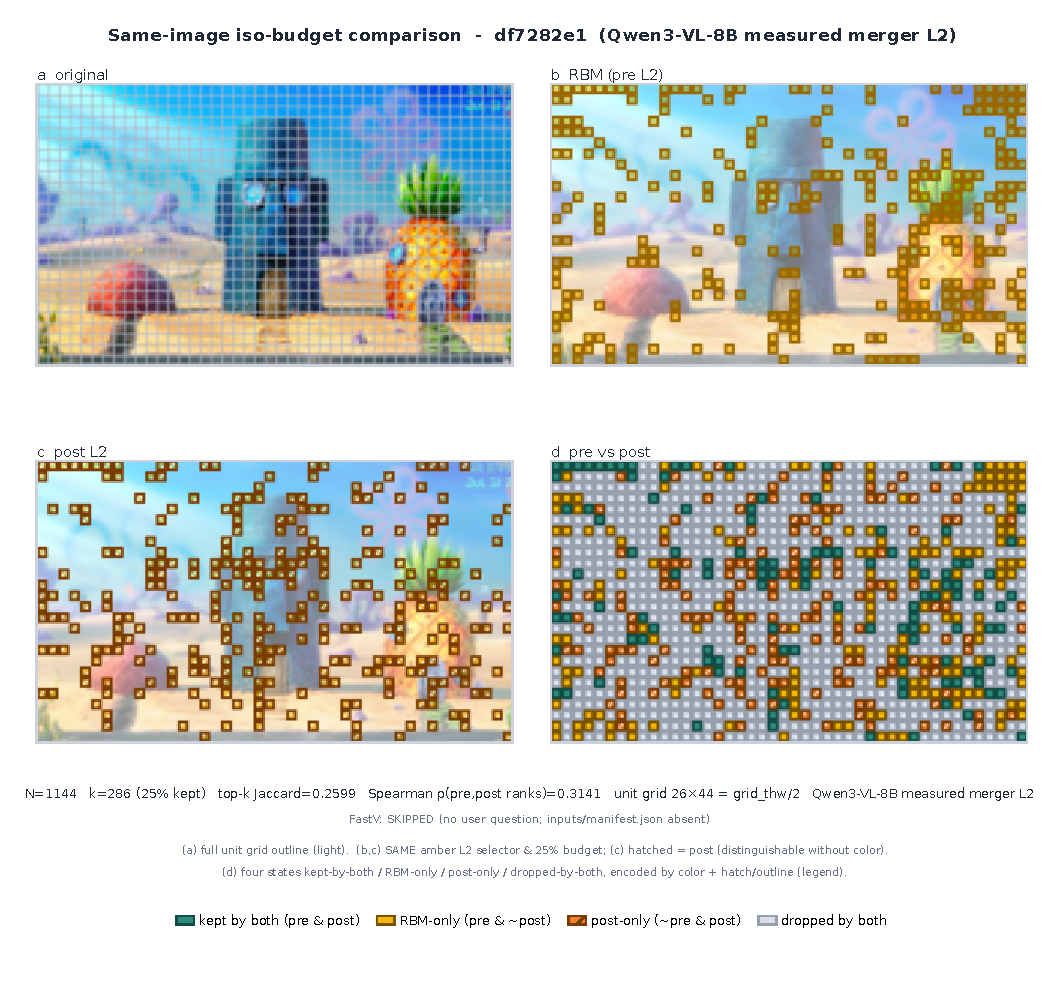
\includegraphics[width=\textwidth]{figs/compare_df7282e1.pdf}
  \caption{Sample \texttt{df7282e1} ($N\!=\!1144$, $k\!=\!286$, $J\!=\!0.260$,
    $\rho\!=\!0.314$). Sparse scene; the four-state map shows RBM-only (amber)
    concentrated on object boundaries while post-only (hatched) scatters over
    flat regions the merger smoothed.}
  \label{fig:cmp_df}
\end{figure*}

\begin{figure*}[p]
  \centering
  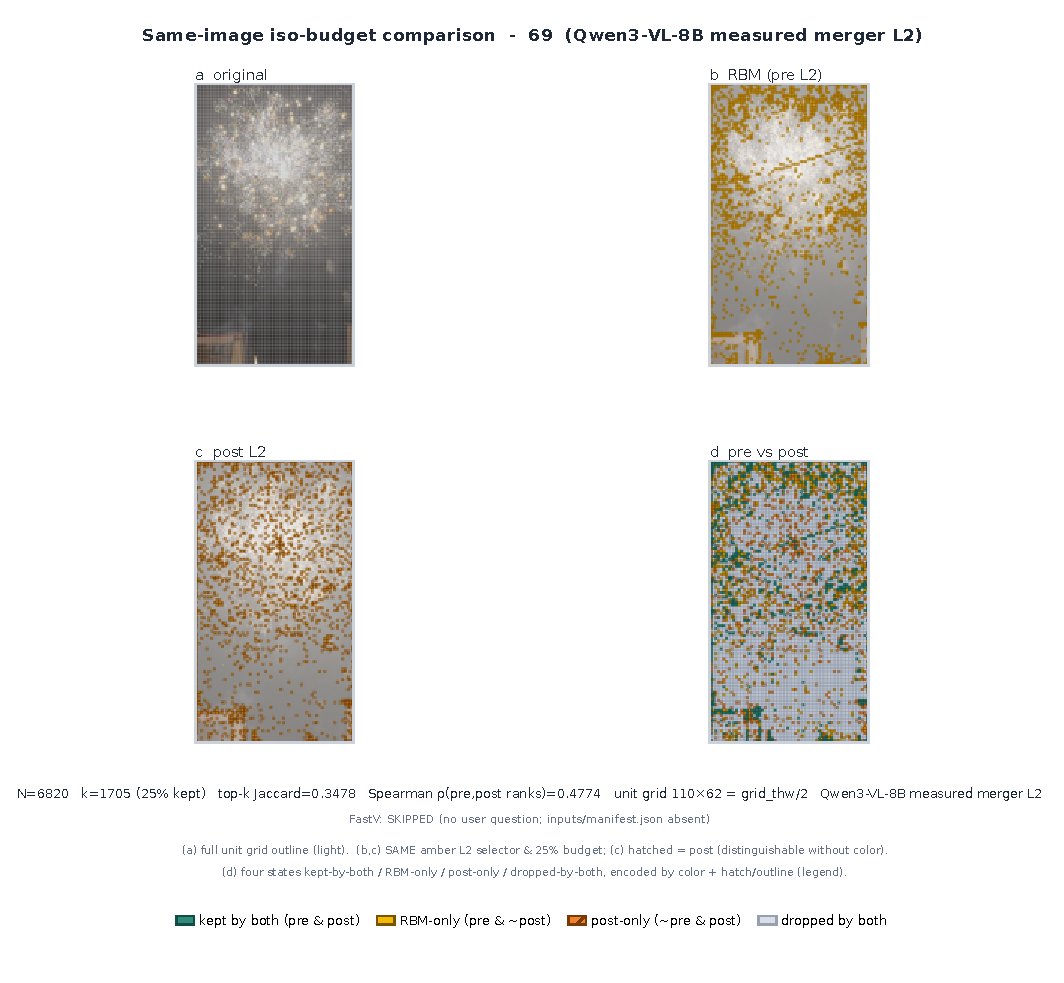
\includegraphics[width=\textwidth]{figs/compare_img69.pdf}
  \caption{Sample \texttt{img69} ($N\!=\!6820$, $k\!=\!1705$, $J\!=\!0.348$,
    $\rho\!=\!0.477$). Highest overlap of the four; the merger preserves more of
    the pre-ranking here, yet two-thirds of the kept set still differs.}
  \label{fig:cmp_69}
\end{figure*}

\begin{figure*}[p]
  \centering
  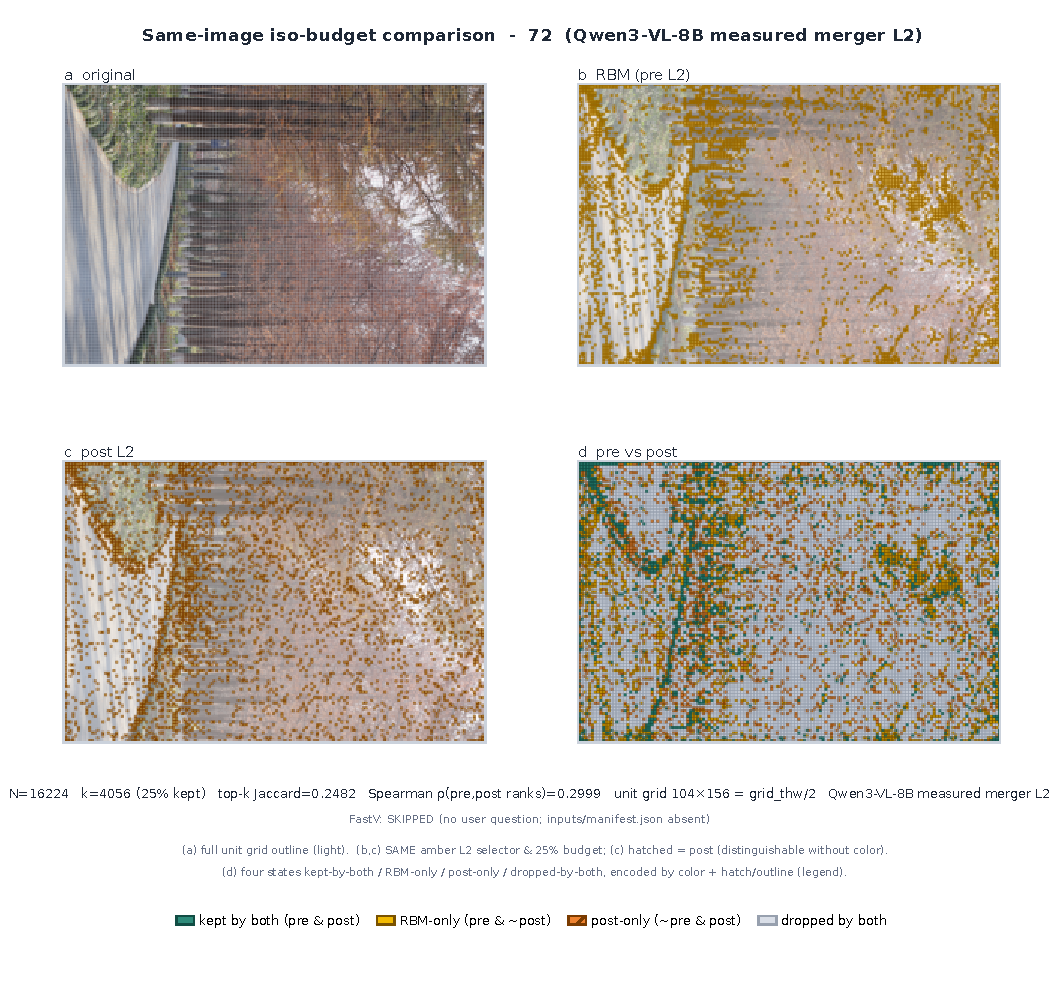
\includegraphics[width=\textwidth]{figs/compare_img72.pdf}
  \caption{Sample \texttt{img72} ($N\!=\!16224$, $k\!=\!4056$, $J\!=\!0.248$,
    $\rho\!=\!0.300$). Textured outdoor scene with a wall edge; the lowest
    overlap --- the merger's lossy aggregation most strongly reorders the
    high-frequency edge vs.\ texture units.}
  \label{fig:cmp_72}
\end{figure*}

\begin{figure*}[p]
  \centering
  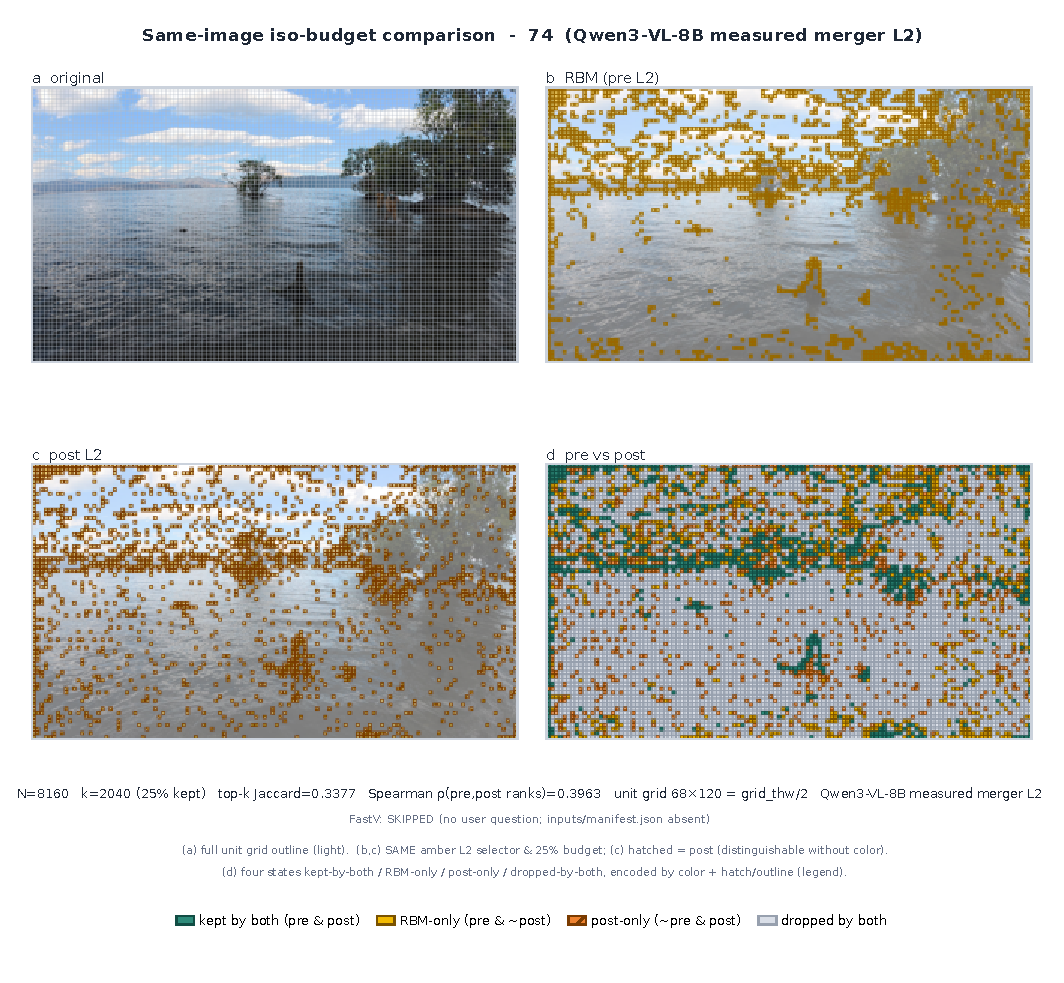
\includegraphics[width=\textwidth]{figs/compare_img74.pdf}
  \caption{Sample \texttt{img74} ($N\!=\!8160$, $k\!=\!2040$, $J\!=\!0.338$,
    $\rho\!=\!0.396$). Waterscape with horizon; RBM-only units track the water
    surface detail that the post-merger L2 demotes in favour of merged sky
    blocks.}
  \label{fig:cmp_74}
\end{figure*}

%──────────────────────────────────────────────────────────────────────────────
\begin{figure*}[p]
\centering
\begin{minipage}{0.86\textwidth}
\section*{S11. Fourth-family gate --- full cell and protocol audit for body Table 2
  (GLM-4.1V-9B-Thinking, $n = 200$)}
\label{app:s11}

This gate tests whether the stage effect transfers to a lineage independent of
Qwen and InternVL. The model uses a GLM-4 text backbone, AIMv2-derived vision
encoder, and a strided $2\!\times\!2$ convolution followed by the
\texttt{Glm4vVisionPatchMerger} MLP. The pre-registered GLM-4.6V-Flash target
could not load because its processor requires transformers $\geq 5.0$rc; the
same-architecture GLM-4.1V fallback was therefore used without a configuration
hack. All nine cells use the same query-blind L2 selector, 25\% retention,
model-default image resolution (effective maximum $\approx 4.82$M pixels),
greedy decoding, and the same thinking-answer parser. Source:
\path{experiments/glm4v_stage_gate.md}; cell JSONs:
\path{runs/glm4v_gate/} (released with code).

\noindent\textbf{Table S11a. Full-precision official scores.}
\begin{center}
  \centering
  \scriptsize
  \begin{tabular}{@{}l l r r r r@{}}
    \toprule
    benchmark & metric & none & pre & post & $\Delta$ (pre$-$post) \\
    \midrule
    TextVQA & VQA-acc     & 0.2417 & 0.2183 & 0.0500 & \textbf{+16.83 pp} \\
    DocVQA  & ANLS        & 0.1039 & 0.1297 & 0.0313 & \textbf{+9.84 pp} \\
    GQA     & exact match & 0.1500 & 0.1600 & 0.1150 & +4.50 pp$^{\dagger}$ \\
    \bottomrule
  \end{tabular}
\end{center}

\noindent\textbf{Table S11b. Token and answer-convergence audit.}
\begin{center}
  \scriptsize
  \begin{tabular}{@{}l r r l@{}}
    \toprule
    benchmark & ptid none & ptid pre/post & boxed none/pre/post \\
    \midrule
    TextVQA & 996.8  & 269.1  & 56/52/15 \\
    DocVQA  & 4868.1 & 1238.8 & 33/30/11 \\
    GQA     & 373.7  & 113.8  & 46/47/39 \\
    \bottomrule
  \end{tabular}
\end{center}

\noindent All cells have $n = 200$ and zero skips. ptid is mean prompt-token
count; pre and post are also exactly equal per sample, not only in the mean.
Boxed counts record samples that reach a final boxed answer within 1024
generated tokens. $^{\dagger}$The GQA direction is protocol-inconclusive and
is not counted as replication.

The prompt-token audit is exact: every paired pre/post example has identical
prompt token ids, and the estimated visual-token counts are approximately
$960\!\to\!233$ (TextVQA), $4830\!\to\!1200$ (DocVQA), and
$347\!\to\!87$ (GQA), with per-image rounding. Thus the large text-dense gaps
cannot be attributed to unequal token budgets. They pass the pre-registered
$5$-pp transfer bar. The other pre-registered half, GQA post$\geq$pre, is not
met: pre exceeds post by 4.5 pp at full $n$, while the $n = 25$ subset where all
three arms reach a boxed answer ties at 0.680/0.680 (pre/post). The latter is a
post-hoc, underpowered diagnostic, not a positive result.

\noindent\textbf{Table S11c. Post-hoc 4096-token diagnostic.}
Cell JSONs: \path{runs/glm4v_gate_v2/} (released with code).
\begin{center}
  \centering
  \scriptsize
  \begin{tabular}{@{}l r r r r r@{}}
    \toprule
    cell & official & contain. & boxed & cut frac. & mean gen. \\
    \midrule
    GQA none     & 0.1650 & 0.290 & 1/200 & 0.740 & 4011 \\
    GQA pre      & 0.1650 & 0.310 & 0/200 & 0.765 & 3997 \\
    GQA post     & 0.1150 & 0.245 & 0/200 & 0.810 & 4057 \\
    TextVQA none & 0.2383 & 0.775 & 2/200 & 0.745 & 3927 \\
    \bottomrule
  \end{tabular}
\end{center}

Increasing max tokens from 1024 to 4096 does not restore greedy convergence:
mean generation remains near the cap and almost no sample reaches a boxed
answer.

The 4096-token probe rules out a short output cap as the source of the GQA
behavior. Its TextVQA containment anchor is $0.775$, close to the published
$\approx 0.77$, while parsed official accuracy remains 0.2383; the model's
visual ability is intact, but deterministic greedy thinking loops rarely
converge to the concise final-answer format. The released model instead
specifies sampling (temperature 0.8, top-$p$ 0.6, top-$k$ 2). We therefore use
this fourth family only as an $n = 200$ replication of the text-dense
pre$\gg$post effect; the full-split claim remains confined to the three model
families in the body, and the GLM GQA direction remains inconclusive.

\par\medskip
\noindent\footnotesize\textbf{Packaging note:} this file converts to the ACM MM
supplementary PDF/archive; run JSONs ship in the code release (anonymous archive
at submission, repository at de-anonymization). Nothing in this supplement
identifies authors, institutions, or repositories (double-blind).
\end{minipage}
\end{figure*}
\clearpage

\end{document}
